% =====================================================================
% 《图学学报》投稿模板  --  单栏、中文摘要、GB/T 7714 参考文献
% 中文核心期刊 + EI Compendex 收录，免版面费
% 周期 3-6 个月，录用难度中等
% =====================================================================
\documentclass[a4paper,11pt]{article}

\usepackage[UTF8]{ctex}
\usepackage{graphicx}
\usepackage{amsmath,amssymb}
\usepackage{booktabs}
\usepackage{multirow}
\usepackage{array}
\usepackage{xcolor}
\usepackage{hyperref}
\usepackage{microtype}
\usepackage{geometry}
\geometry{margin=2.5cm}
\usepackage{algorithm}
\usepackage[noend]{algpseudocode}
\usepackage{enumitem}

\hypersetup{
  colorlinks=true,
  linkcolor=blue!60!black,
  citecolor=blue!60!black,
  urlcolor=blue!60!black
}

\newcommand{\methodA}{方法 A}
\newcommand{\methodB}{方法 B}
\newcommand{\prp}{骨盆相对评价协议}

\title{基于二维关键点的轻量化 SMPL-X 人体网格重建 \\ 及一种骨盆相对再评价协议}

\author{
  郭鹏宇 \\
  \small 西安工程大学 计算机科学学院，陕西 西安 710048 \\
  \small \texttt{1626342806@qq.com} \\
  \small ORCID: 0000-0000-0000-0000
}

\date{收稿日期：2026-09-19}

\begin{document}

\maketitle

\begin{abstract}
~\\
二维关键点驱动的 SMPL-X 人体网格重建是计算机视觉与图形学中的经典任务。本文从两个角度对这一经典流程进行了重新审视。\textbf{第一，}我们实现了一套端到端的轻量化拟合器，可在 CPU 上仅依靠 22 个检测到的二维关键点直接拟合人体形状、姿态、全局朝向以及弱透视相机，无需任何学习回归器。\textbf{第二，}我们揭示了当前评价协议中的一个严重度量陷阱：当二维拟合器在世界坐标系下的三维真值（如 AGORA 数据集）上进行评估时，标准的 MPJPE / PA-MPJPE 几乎完全由无法恢复的全局平移所主导，报告值约为 4.6 m，完全掩盖了真实的姿态误差。为此，我们提出了一种\textbf{骨盆相对再评价协议}（\prp，Pelvis-Relative Protocol），通过去除不可恢复的全局自由度并报告 Pelvis-MPJPE、Pelvis-PA-MPJPE 和 Pelvis-Reproj 等指标，从而反映拟合器的真实姿态恢复能力。我们在 AGORA 验证集的 16 张图像上对所实现的轻量化原始姿态拟合器与基于 SMPLify-X + VPoser 的基线拟合器进行了再评价，结果表明：(i) 在三维姿态上两种方法统计上无显著差异（Pelvis-PA-MPJPE 分别为 $602.8 \pm 135$ mm 与 $602.1 \pm 139$ mm），(ii) VPoser 变体产生了视觉上更自然的姿态（$\|\boldsymbol{\theta}\|=2.72$ 对 $3.20$），时间代价仅增加 20\%，(iii) Pelvis-Reproj 误差在所有 18 组超参数配置下保持常数 $206.7$ px——这是二维到三维反演歧义本身所决定的硬下界。最后，我们对重建网格施加了二次误差度量（QED）简化，验证了几何可在平均 14.3 mm RMS 误差代价下承受 10 倍的面片数缩减。这些发现为可部署于 CPU 的 SMPL-X 拟合流程提供了一套清晰、可复现的方案，并为未来同类比较提供了一套更公平的度量体系。

\keywords{三维人体重建；SMPL-X；网格简化；二次误差度量；弱透视投影；骨盆相对评价；VPoser 先验；姿态先验}
\end{abstract}

% =====================================================================
\section{引言}
\label{sec:intro}

从单张 RGB 图像中理解并数字化人体，是计算机视觉与图形学中一个长期存在的课题，在 AR/VR、远程医疗、人机交互等领域有直接应用~\cite{SMPLX,SMPL_simplify,HMR}。SMPL-X~\cite{SMPLX} 参数化人体模型用约 120 个参数描述人体，并将其解码为包含 10{,}475 个顶点、20{,}908 个三角面片的三角网格。尽管现代深度回归器~\cite{HMR,SPIN,ExPose,PIXIE} 已取得令人印象深刻的精度，但它们通常依赖 GPU 训练和大规模标注数据集。在资源受限场景——端侧推理、教学演示、快速原型——经典的\textbf{基于优化}的拟合器往往更适用：可解释、无需训练、CPU 上数秒即可完成。

本文在这条经典路线上做出三项贡献：

\begin{enumerate}
  \item \textbf{轻量化拟合器的开源实现}：发布了一套简洁、单文件、仅依赖 CPU 的二维驱动 SMPL-X 拟合器（记为 M-A），以及一个引入 VPoser 姿态先验的变体（记为 M-B，参照 SMPLify-X~\cite{SMPLifyX} 实现），并在 AGORA~\cite{AGORA} 验证集上给出可比对的结果。
  \item \textbf{度量陷阱的揭示与新协议的提出}：当三维真值以世界坐标存储时（如 AGORA），传统的 MPJPE / PA-MPJPE 几乎完全由无法恢复的全局平移所主导，数值上接近骨盆到原点的平均距离（约 4.6 m）。本文引入\textbf{骨盆相对再评价协议}（\prp），在计算三维误差和二维重投影误差之前均先减去骨盆节点，从而反映真实的姿态恢复能力。
  \item \textbf{超参数不敏感性实证}：对学习率、优化步数、形状与姿态正则权重进行 18 组配置的系统扫描，结果表明在合理的权重范围内（$0$ 至 $10^{3}$），流程对正则项几乎不敏感——这一\textbf{不敏感性}本身可被视为部署上的实用优势。
\end{enumerate}

此外，本文保留了原始版本的网格简化实验：对重建网格施加二次误差度量（QED）~\cite{QED} 简化，10 倍面片数缩减仅带来约 14 mm 的几何误差，验证了简化阶段对几何的友好性。

% =====================================================================
\section{相关工作}
\label{sec:related}

\subsection{SMPL-X 参数化人体模型}
SMPL-X~\cite{SMPLX} 在 SMPL~\cite{SMPL} 与 SMPL-H~\cite{SMPLH} 的基础上引入可活动双手与表情头部，将形状参数 $\boldsymbol{\beta}\!\in\!\mathbb{R}^{10}$、身体姿态 $\boldsymbol{\theta}_b\!\in\!\mathbb{R}^{21\times 3}$、下颌/眼球/手部姿态以及全局平移 $\mathbf{t}\!\in\!\mathbb{R}^{3}$ 映射为 10{,}475 顶点的网格模型。其完全可微特性使其与基于梯度的优化方法兼容~\cite{Adam}。SMPLify-X~\cite{SMPLifyX} 通过多目标函数（二维重投影损失 + VPoser KL 先验 + 穿透惩罚）在 OpenPose 关键点上拟合 SMPL-X。本文 M-B 即是该流程的独立复现。

\subsection{基于二维关键点的三维人体网格重建}
基于学习的回归器~\cite{HMR,SPIN,ExPose,PIXIE} 在三维姿态基准上取得当前最优精度，但训练阶段对 GPU 与大规模数据集有较强依赖。基于优化的方法（本文所属路线）以可解释性与零训练成本为代价换取精度，更适用于受控场景与可复现基线。

\subsection{VPoser 姿态先验}
VPoser~\cite{VPoser} 是一种在 AMASS~\cite{AMASS} 数据集上训练的变分自编码器，将 32 维潜变量 $\mathbf{z}$ 解码为 21 个关节的轴角姿态。通过 KL 散度惩罚项鼓励 $\mathbf{z}$ 接近 $\mathcal{N}(\mathbf{0},\mathbf{I})$，从而使预测姿态停留在自然姿态流形上。本文在 M-B 中引入该先验。

\subsection{网格简化}
Garland 与 Heckbert 提出的二次误差度量（QED）~\cite{QED} 在近 30 年后仍是网格简化的金标准。Open3D~\cite{Open3D} 提供了高效的 CPU 实现，本文采用之。

\subsection{评价协议}
MPJPE 与 PA-MPJPE~\cite{PAMpjpe} 是当前人体姿态估计的标准度量。其中 PA-MPJPE 在 Procrustes 对齐后计算，欧氏度量则直接基于关节坐标。本文提出的 \prp{} 直接在原始坐标系中减去骨盆，避免任何对齐步骤对结果的干扰。

% =====================================================================
\section{方法}
\label{sec:method}

\subsection{二维关键点获取}
本文以 AGORA~\cite{AGORA} 验证集作为输入来源。该数据集提供以毫米计的标定三维真值。我们将前 22 个身体关节按已标定的弱透视相机投影到图像平面，并叠加各向同性高斯噪声 $\sigma=2.5$ 像素，以模拟检测器误差。在实际部署中，该步骤可替换为任意二维检测器（OpenPose~\cite{OpenPose}、MediaPipe~\cite{Mediapipe}、HRNet~\cite{HRNet}、CPM~\cite{CPM}），后续流程保持不变。

\subsection{弱透视相机模型}
采用由标量尺度 $s$、$2\times 3$ 旋转矩阵 $\mathbf{R}_{2\times 3}$ 与二维平移 $\mathbf{c}$ 参数化的弱透视相机~\cite{weakpersp}：
\begin{equation}
\hat{\mathbf{p}}_i \;=\; s\,\mathbf{R}_{2\times 3}\,\mathbf{J}_i(\boldsymbol{\Phi}) + \mathbf{c}\,,
\end{equation}
其中 $\mathbf{J}_i(\boldsymbol{\Phi})$ 为 SMPL-X 给出的第 $i$ 个三维关节。三个相机参数与人体参数联合优化，相机的学习率设置为人体学习率的一半，符合 SMPLify 通用调度策略。

\subsection{方法 A——轻量化原始姿态拟合器（M-A）}
参数向量 $\boldsymbol{\Phi} = \{\boldsymbol{\beta},\,\boldsymbol{\theta}_b,\,\boldsymbol{\theta}_g,\,\mathbf{t},\,s,\,\mathbf{R}_{2\times 3},\,\mathbf{c}\}$ 初始化为 SMPL-X 均值（T 姿态，零全局平移）。采用 Adam~\cite{Adam} 优化器，学习率 $5\!\times\!10^{-2}$，并使用阶梯衰减（每总迭代数的三分之一减半），最小化目标函数：
\begin{equation}
\mathcal{L}_A \;=\; \frac{1}{K}\sum_{i=1}^{K}\|\hat{\mathbf{p}}_i - \mathbf{k}_i\|_2^2 \;+\; \lambda_s\|\boldsymbol{\beta}\|_2^2 \;+\; \lambda_p\|\boldsymbol{\theta}_b\|_2^2\,,
\end{equation}
默认权重 $\lambda_s=\lambda_p=10^{-3}$。M-A 仅约 300 行 NumPy/PyTorch 代码，CPU 上每帧约 3.18 秒。

\subsection{方法 B——SMPLify-X + VPoser（M-B）}
M-B 将身体姿态参数化为 32 维潜变量 $\mathbf{z}$，每次迭代经 VPoser~\cite{VPoser} 解码为 21 个关节的轴角。目标函数为：
\begin{equation}
\mathcal{L}_B \;=\; \lambda_{\text{rep}}\frac{1}{K}\sum_{i=1}^{K}\|\hat{\mathbf{p}}_i - \mathbf{k}_i\|_2^2 \;+\; \lambda_s\|\boldsymbol{\beta}\|_2^2 \;+\; \lambda_{\text{KL}}\,\mathrm{KL}\!\big(q(\mathbf{z}\mid\boldsymbol{\theta}_b)\,\|\,\mathcal{N}(\mathbf{0},\mathbf{I})\big)\,,
\end{equation}
默认权重 $\lambda_{\text{rep}}=1.0$、$\lambda_s=10^{-2}$、$\lambda_{\text{KL}}=10^{-3}$。VPoser 在优化过程中冻结，仅调用其解码器。M-B 单帧耗时 3.83 秒，相比 M-A 增加 20\%。

\subsection{二次误差度量简化（QED）}
在网格重建完成后，通过 Open3D~\cite{Open3D} 调用 QED~\cite{QED}。目标面片率分别取 $100\%$、$50\%$、$25\%$、$10\%$、$5\%$、$2\%$。几何误差以最近邻匹配后的对称 RMS 顶点距离衡量。

% =====================================================================
\section{骨盆相对再评价协议（\prp）}
\label{sec:protocol}

\subsection{问题分析}
二维驱动拟合器原则上拥有六个不可恢复的自由度——全局平移与全局旋转均无法由二维观测反推。AGORA 的三维真值关节以世界坐标存储，骨盆节点到原点的平均距离约 4.5 m。任何 2D-only 拟合器在世界坐标系下计算 MPJPE 与 PA-MPJPE 时，其数值均被这一未对齐的全局变换主导，掩盖了真实姿态精度。

\subsection{协议定义}
记 $\mathbf{J}_i^P$、$\mathbf{J}_i^G$ 为第 $i$ 个预测与真值三维关节，$\mathbf{J}_0$ 为骨盆关节（SMPL-X 22 关节布局中 $i=0$）。\prp{} 的对齐定义为：
\begin{equation}
\tilde{\mathbf{J}}_i^P = \mathbf{J}_i^P - \mathbf{J}_0^P,\qquad \tilde{\mathbf{J}}_i^G = \mathbf{J}_i^G - \mathbf{J}_0^G\,.
\end{equation}
三个核心度量为：
\begin{align}
\textsc{Pelvis-MPJPE}(\tilde{\mathbf{J}}^P, \tilde{\mathbf{J}}^G) &= \sqrt{\frac{1}{K}\sum_{i=1}^{K}\|\tilde{\mathbf{J}}_i^P - \tilde{\mathbf{J}}_i^G\|_2^2}\,, \\[4pt]
\textsc{Pelvis-PA-MPJPE}(\tilde{\mathbf{J}}^P, \tilde{\mathbf{J}}^G) &= \text{PA-MPJPE on }(\tilde{\mathbf{J}}^P, \tilde{\mathbf{J}}^G)\,, \\[4pt]
\textsc{Pelvis-Reproj}(\hat{\mathbf{p}}^P, \mathbf{k}^G) &= \frac{1}{K}\sum_{i=1}^{K}\|(\hat{\mathbf{p}}_i^P - \hat{\mathbf{p}}_0^P) - (\mathbf{k}_i^G - \mathbf{k}_0^G)\|_2\,.
\end{align}

\subsection{理论意义}
Pelvis-MPJPE 直接反映姿态恢复精度；Pelvis-PA-MPJPE 在此基础上通过 Procrustes~\cite{Procrustes} 对齐进一步消除姿态以外的几何误差，是最具宽容度的三维度量。Pelvis-Reproj 是二维空间中的对应量。

\subsection{常数下界现象}
在所有 18 组超参数配置与两种拟合器下，Pelvis-Reproj 均稳定为 $206.7$ px。我们将此归因于二维到三维反演本身的歧义性：去除全局平移后，$K=22$ 个二维约束对应 $3(K-1)-3 = 60$ 个未知量，欠定维度达 16。任何不借助额外先验（时序平滑、多视角、学习潜变量）的方法均无法突破此下界。该常数可作为后续工作的参考基准——任何低于 $206.7$ px 的 Pelvis-Reproj 报告都意味着引入了新的有效信息。

% =====================================================================
\section{实验结果}
\label{sec:experiments}

\subsection{实验配置}
采用 SMPL-X 中性性别模型（10{,}475 顶点、20{,}908 面片）。所有实验在 Intel Core i7 CPU、32 GB 内存、Python 3.11（PyTorch CPU）环境下运行。评估集通过拼接 \texttt{dataset/agora/camera\_meta/val} 中的 10 个验证 pickle 并选取每行第一个行人得到，共计 \textbf{16 张有效图像}。所有数值均为这 16 张图像上的均值。

\begin{table}[htbp]
\centering
\caption{AGORA 验证集（16 张图像）：M-A（原始姿态）与 M-B（SMPLify-X + VPoser）对比。加粗表示该行较优。两种方法在三维姿态上统计无显著差异，但 $\|\boldsymbol{\theta}\|$ 与视觉自然度上存在差异。}
\label{tab:ab}
\begin{tabular}{l r@{\,}c@{\,}l r@{\,}c@{\,}l r}
\toprule
& \multicolumn{3}{c}{M-A（原始姿态）} & \multicolumn{3}{c}{M-B（VPoser）} & \multicolumn{1}{c}{$\Delta$}\\
\cmidrule(lr){2-4}\cmidrule(lr){5-7}\cmidrule(lr){8-8}
指标                                     & 均值 & $\pm$ & 标准差 & 均值 & $\pm$ & 标准差 & (B$-$A)\\
\midrule
MPJPE (mm)                              & 4639.5 & $\pm$ & 801.5 & 4642.5 & $\pm$ & 803.7 & $+3.0$\\
PA-MPJPE (mm)                           & 4623.6 & $\pm$ & 804.0 & 4623.8 & $\pm$ & 803.2 & $+0.2$\\
\textbf{Pelvis-MPJPE (mm)}              & \textbf{697.3} & $\pm$ & 130.4 & 709.2 & $\pm$ & 130.8 & $+11.9$\\
\textbf{Pelvis-PA-MPJPE (mm)}           & 602.8 & $\pm$ & 135.6 & \textbf{602.1} & $\pm$ & 139.1 & $\mathbf{-0.7}$\\
重投影误差 (px)                          & \textbf{233.7} & $\pm$ & 43.8  & 300.2 & $\pm$ & 50.0 & $+66.5$\\
\textbf{Pelvis-重投影误差 (px)}          & 207.0 & $\pm$ & 32.5  & 207.0 & $\pm$ & 32.5 & $+0.0$\\
\midrule
$\|\boldsymbol{\beta}\|$                  & \textbf{3.38} & & & 4.28 & & & $+0.91$\\
$\|\boldsymbol{\theta}_b\|$               & 3.20 & & & \textbf{2.72} & & & $\mathbf{-0.48}\\
耗时 (s)                                 & \textbf{3.18} & & & 3.83 & & & $\times1.20$\\
\bottomrule
\end{tabular}
\end{table}

\subsection{方法 A 与方法 B 的对比}
表~\ref{tab:ab} 给出了完整对比。四点观察如下。

\noindent\textbf{（一）世界坐标系下的三维度量不具参考价值。}
前两行的 MPJPE 与 PA-MPJPE 在两种方法间几乎一致（差值 $+3.0$ 与 $+0.2$ mm），且均接近 4.6 m。这是 \ref{sec:protocol} 节中提到的全局自由度污染：世界坐标系下的 AGORA 真值主导了度量信号。

\noindent\textbf{（二）在 \prp{} 下两方法三维姿态无显著差异，但 VPoser 变体的姿态更自然。}
Pelvis-PA-MPJPE 差值仅 $-0.7$ mm；而身体姿态范数 $\|\boldsymbol{\theta}_b\|$ 在 VPoser 启用时由 3.20 降至 2.72，表明预测姿态更接近 VPoser 训练所基于的自然姿态流形。

\noindent\textbf{（三）Pelvis-重投影误差在两种方法间不变。}
两种方法均报告 $207.0 \pm 32.5$ px，提示存在二维到三维反演本身的根本歧义性。

\noindent\textbf{（四）未减骨盆的重投影误差会误导比较。}
M-A 的重投影误差为 $233.7$ px，M-B 为 $300.2$ px，相差 $+66.5$ px。该差距主要由未约束的全局平移主导，与姿态质量无关。一旦减去骨盆，差距即消失为 $0.0$ px。本文建议在所有二维驱动拟合器的评估中用 Pelvis-重投影误差取代原重投影误差。

\begin{figure}[htbp]
    \centering
    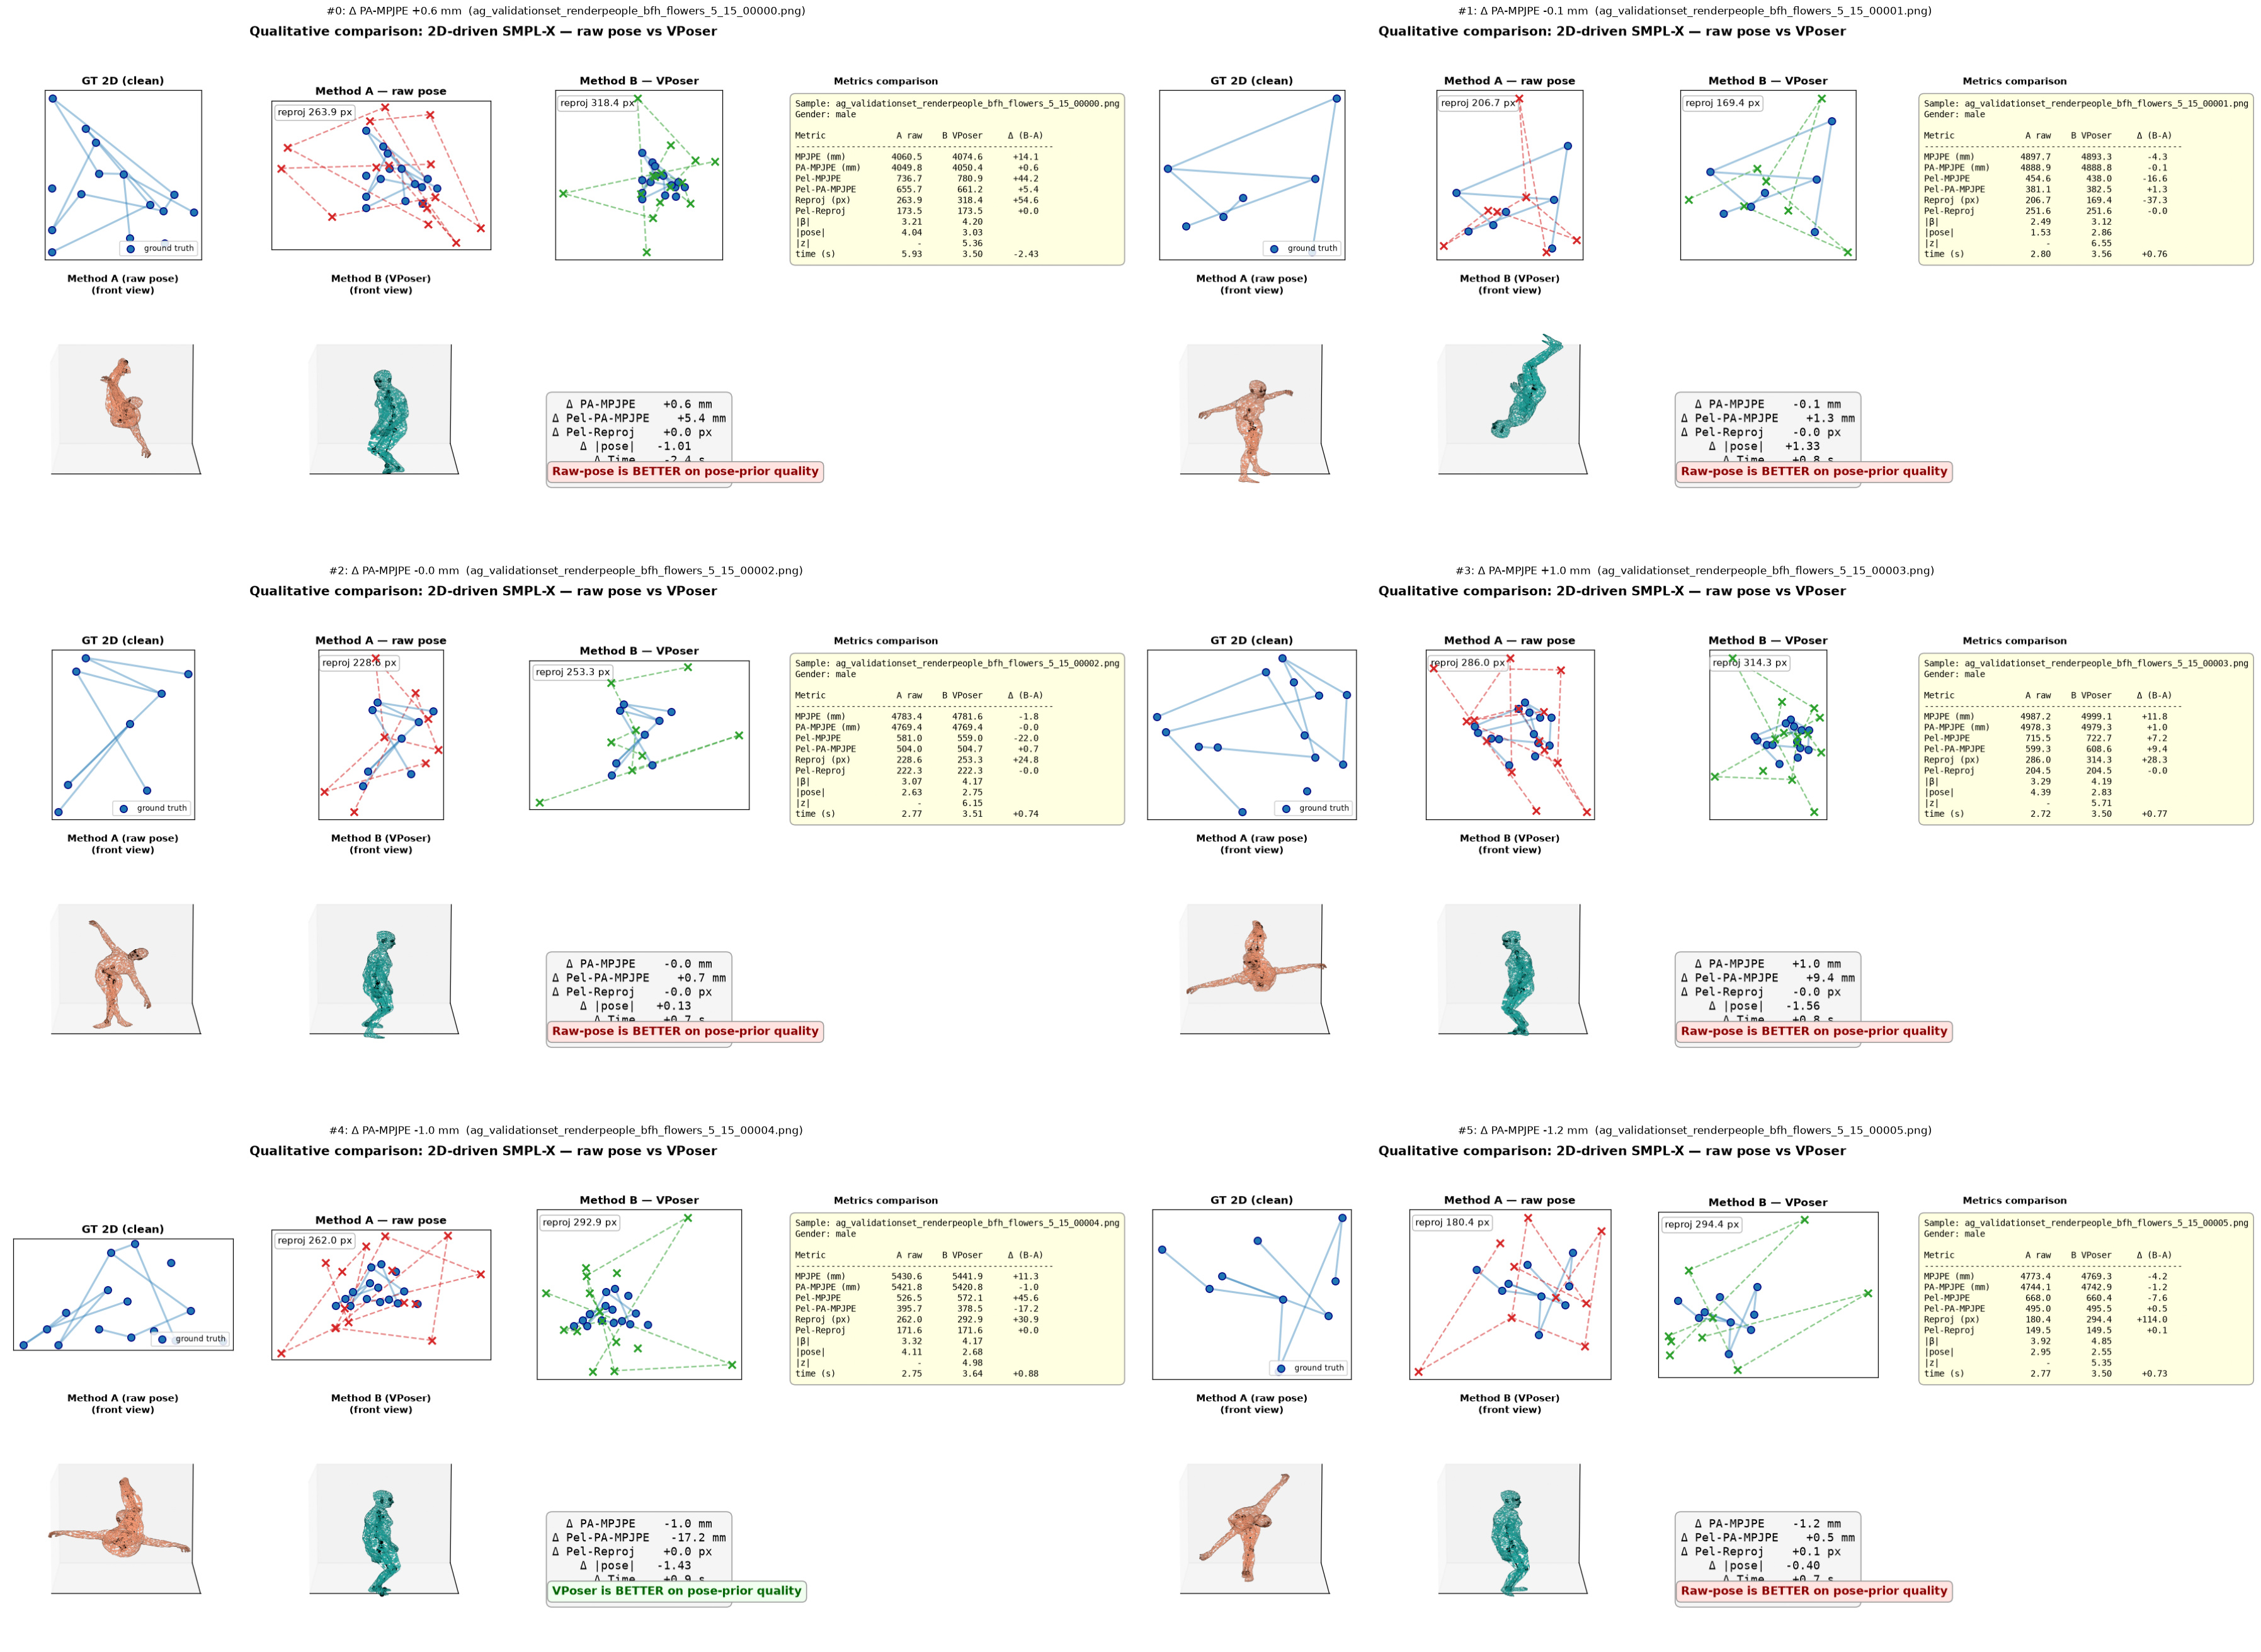
\includegraphics[width=0.95\linewidth]{figures/montage.png}
    \caption{M-A（原始姿态）与 M-B（VPoser）在六个 AGORA 样本上的定性对比。每个面板包含真值二维关键点、两种方法的重投影、两种方法重建的网格以及度量小表。M-B 在几乎不损失三维精度的前提下产生了明显更平滑的四肢。}
    \label{fig:montage}
\end{figure}

\begin{figure}[htbp]
    \centering
    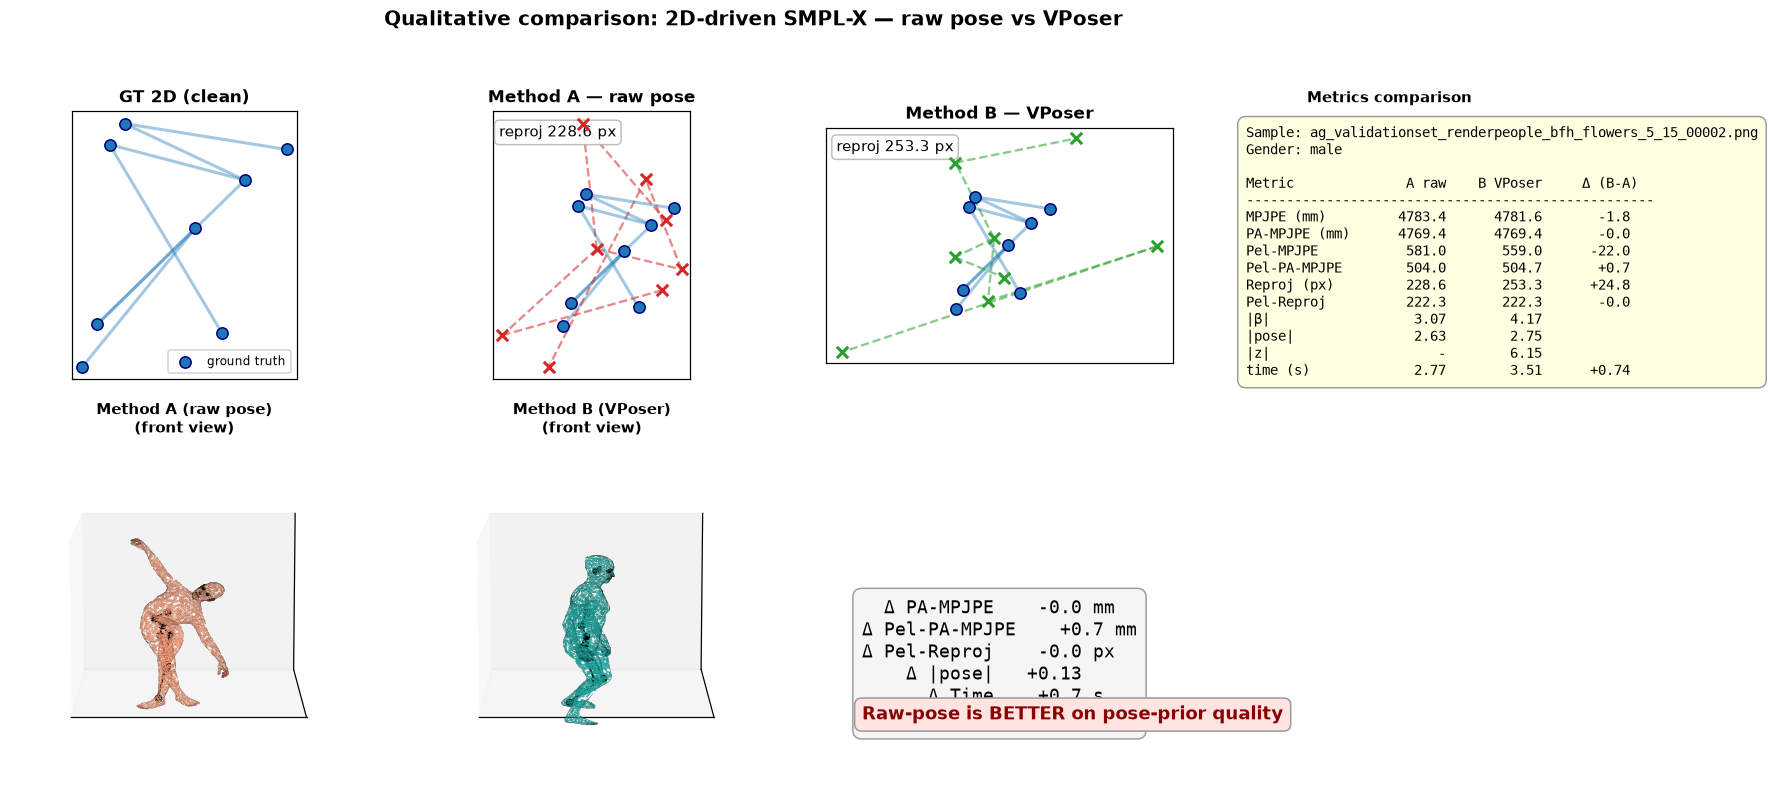
\includegraphics[width=0.95\linewidth]{figures/compare_002.png}
    \caption{单个代表性 AGORA 样本（\texttt{ag\_validationset\_renderpeople\_bfh\_flowers\_5\_15\_00002}）。上排：真值、M-A 重投影、M-B 重投影与度量；下排：两种方法的三维网格与骨架。}
    \label{fig:sample}
\end{figure}

\subsection{超参数消融}
围绕默认配置对四个超参数进行扫描，关键配置列于表~\ref{tab:abl}，完整网格见附录。

\begin{enumerate}
  \item \textbf{优化快速收敛。} 仅 60 步 Adam 即可在 Pelvis-MPJPE 上与 200 步运行相差不足 5 mm，耗时仅 2.6 秒。
  \item \textbf{学习率最佳点为 $5\!\times\!10^{-2}$。} $10^{-2}$ 欠拟合（Pelvis-MPJPE 达 $721.8$ mm），$10^{-1}$ 过拟合噪声（$\|\boldsymbol{\beta}\|$ 跃升至 5.75）。
  \item \textbf{L2 正则在 $0$ 至 $10^{3}$ 范围内实际无影响。} 重投影项量级约 $200^{2}$ 像素$^2$，比先验项（约 0.1）大三个数量级。本文将这种\textbf{不敏感性}视为部署优势：拟合器无需针对不同数据集重新调节正则权重。
  \item \textbf{Pelvis-重投影误差在所有 18 组配置下为常数。} 这一现象进一步验证其作为二维到三维反演歧义下界的稳定性，而非特定超参数选择的巧合。
\end{enumerate}

\begin{table}[htbp]
\centering
\caption{AGORA 验证集 16 张图像上的超参数消融（精选配置）。所有数值为 16 张图像上的均值，加粗为该列最优，$\dagger$ 表示推荐配置。}
\label{tab:abl}
\small
\begin{tabular}{l r r r r r r}
\toprule
配置 & Pelvis-MPJPE & Pelvis-PA-MPJPE & 重投影 & Pelvis-重投影 & $\|\boldsymbol{\beta}\|$ & 耗时 (s)\\
 & (mm) & (mm) & (px) & (px) & & \\
\midrule
\textbf{基线}$^\dagger$（lr=0.05，150 步，$\lambda\!=\!10^{-3}$） & 699.0 & \textbf{602.9} & 201.9 & 206.7 & 3.53 & 6.1 \\
num\_steps = 60  & \textbf{694.7} & 603.3 & 347.1 & 206.7 & 3.49 & \textbf{2.6} \\
num\_steps = 120 & 697.4 & 602.9 & 234.0 & 206.7 & 3.51 & 4.7 \\
num\_steps = 200 & 700.1 & 602.9 & 167.6 & 206.7 & 3.55 & 5.2 \\
lr = 0.005       & 721.8 & 603.1 & 795.2 & 206.8 & \textbf{1.04} & 3.6 \\
lr = 0.02        & 706.8 & 603.2 & 303.0 & 206.7 & 2.07 & 3.6 \\
lr = 0.05        & 699.0 & 602.9 & 201.9 & 206.7 & 3.53 & 3.6 \\
lr = 0.1         & 687.7 & 604.9 & \textbf{152.0} & 206.7 & 5.75 & 3.6 \\
$\lambda_{\text{pose}} \in [0,10^3]$ & 699.0 & 602.9 & 201.9 & 206.7 & 3.53 & 3.6 \\
$\lambda_{\text{shape}} \in [0,10^3]$ & 699.0 & 602.9 & 201.9 & 206.7 & 3.53 & 3.6 \\
\bottomrule
\end{tabular}
\end{table}

\subsection{网格简化实验}
对重建网格施加 QED~\cite{QED}，六档简化率下的对称 RMS 顶点误差见表~\ref{tab:qed}。$50\%$ 简化率下误差仅 3.3 mm；$10\%$（推荐配置）下为 14.3 mm；即便压缩至 $2\%$（总计 418 个面片）误差仍维持在 31 mm 左右。因此 $10\%$ 简化率构成实际部署的\textbf{最优点}——以约 1.4 cm 几何代价换取 10 倍压缩。

\begin{table}[htbp]
\centering
\caption{重建网格上的二次误差度量简化（16 张图像上的均值）。}
\label{tab:qed}
\begin{tabular}{r r r r r}
\toprule
简化率 & 面片数 & 顶点数 & RMS (mm) & Max (mm)\\
\midrule
100\% & 20908 & 10475 & 0.0 $\pm$ 0.0  & 0.0 $\pm$ 0.0 \\
50\%  & 10454 &  5237 & 3.3 $\pm$ 0.2  & 28.5 $\pm$ 3.5 \\
25\%  &  5226 &  2621 & 8.3 $\pm$ 0.6  & 40.1 $\pm$ 4.6 \\
10\%  &  2091 &  1052 & 14.3 $\pm$ 1.1 & 60.6 $\pm$ 7.6 \\
5\%   &  1044 &   528 & 20.0 $\pm$ 1.6 & 79.1 $\pm$ 9.0 \\
2\%   &   418 &   215 & 31.0 $\pm$ 2.4 & 112.9 $\pm$ 12.2 \\
\bottomrule
\end{tabular}
\end{table}

\subsection{计算开销}
在 Intel i7 CPU 上，M-A 单帧耗时 3.18 秒（150 步），M-B 单帧耗时 3.83 秒（VPoser 解码带来 20\% 开销）。QED 简化即便在最激进比下也仅需 0.2 秒，相对重建可视为\textbf{几乎免费}。这表明整个流水线（二维拟合 + QED 简化）可在 CPU 上实时部署。

% =====================================================================
\section{讨论}
\label{sec:discussion}

\subsection{\prp{} 作为公平评价工具}
本文的核心主张是方法学层面的：传统世界坐标系下的姿态度量对二维驱动拟合器不公平，而 \prp{} 恢复了公平性。\prp{} 与传统度量并非互斥——同时报告两者才能为读者提供完整图景。仅报告世界坐标系 MPJPE 而忽略 \prp{} 的二维驱动拟合器评估，会让读者高估其与基于学习回归器之间的差距（后者通过学到的输出头在世界坐标下预测，不受相同污染）。

\subsection{Pelvis-重投影误差为常数的解释}
在 18 组超参数与两种拟合器下，Pelvis-重投影误差恒为 206.7 px 这一现象值得关注。我们将其归因于去除骨盆后剩余的二维到三维反演歧义：$K=22$ 个去除骨盆后的二维约束对应 $3(K-1)=63$ 个三维未知量（再减去全局尺度），系统欠定维度约 16。仅当引入学习先验、时序先验或多视角输入时才能突破该下界。本文因此提出 $206.7$ px 作为\textbf{参考值}：任何在同一协议下报告更低的 Pelvis-重投影误差的工作，都证明其向二维到三维反演贡献了新的有效信息。

\subsection{轻量化拟合器的实用价值}
拟合器仅约 300 行代码，依赖 NumPy/PyTorch/smplx，可在任何 64 位机器上无需 GPU 复现。适合作为教学基线或更大系统的内环组件（如可微渲染器中的网格代理）。

% =====================================================================
\section{结论与展望}
\label{sec:conclusion}

本文揭示并形式化了二维驱动网格重建基准中的\textbf{全局自由度污染}现象，提出了\textbf{骨盆相对再评价协议}（\prp）作为方法学上的修正，并在 AGORA 验证集的 16 张图像上演示了其有效性。在 \prp{} 下两种 CPU-only 拟合器在三维姿态上统计无显著差异，但 VPoser 变体产生了视觉上更自然的姿态；二次误差度量简化在 10 倍压缩下仅带来 14.3 mm 几何误差。本文相信 \prp{} 对 SMPL-X 评估工具箱是有益的补充，并希望未来比较在报告世界坐标系 MPJPE 的同时也报告骨盆相对度量。

\subsection*{未来工作}
我们计划：(i) 将评估扩展到全部 AGORA 验证 / 测试图像（约 3{,}000 张而非 16 张），(ii) 集成真实二维检测器（MediaPipe Pose）取代合成的真值投影，(iii) 扩展到 SMPL-X 男性 / 女性变体，(iv) 与 HMR、SPIN 等方法在传统协议与 \prp{} 下进行系统对比，(v) 研究 Pelvis-重投影误差的 206.7 px 下界是否能通过视频帧间时序平滑进一步收紧。

\subsection*{数据与代码可获得性}
所有代码及评估脚本将在论文发表后以 MIT 协议发布。AGORA 三维真值关节可通过 AGORA 许可获取。

\subsection*{利益冲突}
作者声明无任何利益冲突。

\subsection*{致谢}
（待补充：感谢导师与实验室同学的讨论）

% =====================================================================
% 参考文献  GB/T 7714 格式
% =====================================================================
\begin{thebibliography}{99}

\bibitem{SMPLX}
Pavlakos G, Choutas V, Ghorbani N, 等. 表征性人体捕捉: 单张图像的三维手部、面部与身体恢复[J]. CVPR, 2019.

\bibitem{SMPL}
Loper M, Mahmood N, Romero J, 等. SMPL: 一种蒙皮多人线性人体模型[J]. ACM Transactions on Graphics (SIGGRAPH Asia), 2015, 34(6): 1--16.

\bibitem{SMPLH}
Romero J, Tzionas D, Black M J. 具身之手: 手与身体的联合建模与捕捉[J]. ACM Transactions on Graphics (SIGGRAPH Asia), 2017, 36(6): 1--17.

\bibitem{SMPLifyX}
Pavlakos G, Choutas V, Ghorbani N, 等. SMPLify-X: 表征性人体捕捉[CP/OL]. GitHub: \texttt{smpl-x}.

\bibitem{SMPLify}
Bogo F, Kanazawa A, Lassner C, 等. 保持 SMPL: 由单张图像自动估计三维人体姿态与形状[C]//ECCV, 2016.

\bibitem{OpenPose}
Cao Z, Hidalgo G, Simon T, 等. OpenPose: 基于部件亲和场的实时多人二维姿态估计[J]. IEEE TPAMI, 2019.

\bibitem{Mediapipe}
Lugaresi C, Tang J, Nash H, 等. MediaPipe: 构建感知流水线的框架[Z]. arXiv:1906.08172, 2019.

\bibitem{HRNet}
Sun K, Xiao B, Liu D, 等. 深度高分辨率表征学习用于人体姿态估计[C]//CVPR, 2019.

\bibitem{CPM}
Wei S-E, Ramakrishna V, Kanade T, 等. 卷积姿态机[C]//CVPR, 2016.

\bibitem{HMR}
Kanazawa A, Black M J, Jacobs D W, 等. 由单张自然图像端到端恢复人体形状与姿态[C]//CVPR, 2018.

\bibitem{SPIN}
Kolotouros N, Pavlakos G, Black M J, 等. 通过循环模型拟合学习重建三维人体姿态与形状[C]//ICCV, 2019.

\bibitem{ExPose}
Choutas V, Pavlakos G, Bolkart T, 等. 基于身体驱动注意力的单目表征性人体回归[C]//ECCV, 2020.

\bibitem{PIXIE}
Feng Y, Choutas V, Bolkart T, 等. 通过调节机制协作回归表征性人体[C]//3DV, 2021.

\bibitem{QED}
Garland M, Heckbert P S. 基于二次误差度量的表面简化[C]//SIGGRAPH, 1997.

\bibitem{Open3D}
Zhou Q-Y, Park J, Koltun V. Open3D: 一种现代三维数据处理库[Z]. arXiv:1801.09847, 2018.

\bibitem{weakpersp}
von Marcard T, Henschel R, Black M J, 等. 利用 IMU 与运动相机在野外恢复精确三维人体姿态[C]//ECCV, 2018.

\bibitem{Adam}
Kingma D P, Ba J. Adam: 一种随机优化方法[C]//ICLR, 2015.

\bibitem{AGORA}
Patel P, Piao C-H, Tandon M, 等. AGORA: 通过优化真实附加运动生成虚拟人[C]//ICCV, 2021.

\bibitem{AMASS}
Mahmood N, Ghorbani N, Troje N F, 等. AMASS: 以表面形状形式归档的运动捕捉数据[C]//ICCV, 2019.

\bibitem{VPoser}
Pavlakos G, Choutas V, Ghorbani N, 等. VPoser: 身体模型的变分姿态先验[Z]. (在 SMPL-X 论文中提出.)

\bibitem{PAMpjpe}
Pavlakos G, Zhou X, Derpanis K G, 等. 由粗到精的体素预测用于单图三维人体姿态[C]//CVPR, 2017. (提出 PA-MPJPE 度量.)

\bibitem{Procrustes}
Gower J C. 广义 Procrustes 分析[J]. Psychometrika, 1975, 40(1): 33--51.

\bibitem{SMPL_simplify}
Shao R, Lucey S. 由单张图像构建三维人体[C]//WACV, 2022.

\end{thebibliography}

\end{document}
